\section{The System}
\label{sec.thesystem}

\subsection{Requirements}
\label{sec.thesystem_req}
The system represents a web shop and the main requirements are to:
\begin{itemize}
  \item \emph{Registration} - the customer should be able to registerand create
  a valid profile using an email (as userid), password, name and delivery info: address,
  zip code, and phone number. (The fields should be validated: valid email
  address - validation sent by email; password should have at least six
  characters, al least one digit, one letter and at least one
  non-digit/non-letter character; zip code should be 4 digit; phone number
  should be 8 digit number).
  \item \emph{Browsing} - the customer should be able to browse a list of pizzas
  with description and price for each. The list should be sorted either after
  name or price.
  \item \emph{Basket} - the customer should be able to add/remove pizzas
  to/from a shopping chart. It should see the quantities and price per product
  along with the total price of the pizzzas in the basket.
  \item \emph{Checkout} - the customer should be able to checkout a basket
  (verify the contents and confirm purchase).
  \item \emph{Admin} - An administrator should be able to log in, manage the
  list of pizzas (add/remove).
\end{itemize}
\subsection{Design and Implementation}
\label{sec.thesystem.design_impl}

\subsubsection{JSP}
\label{sec.thesystem.jsp}
The overall system design is built on the MVC (Model View Controller) design
pattern. The key motivation behind this approach is to separate the code that
creates and manipulates data from the code that presenfts the data. The
\emph{model} encapsulates data representation (beans). The \emph{controller}
manages the interactions with the clients, deciding which JSP page should
present the results. The \emph{view}provides the appropiate views for the
clients. Figure illustrates the basic design:

 \begin{figure}[H]
    \begin{center}
        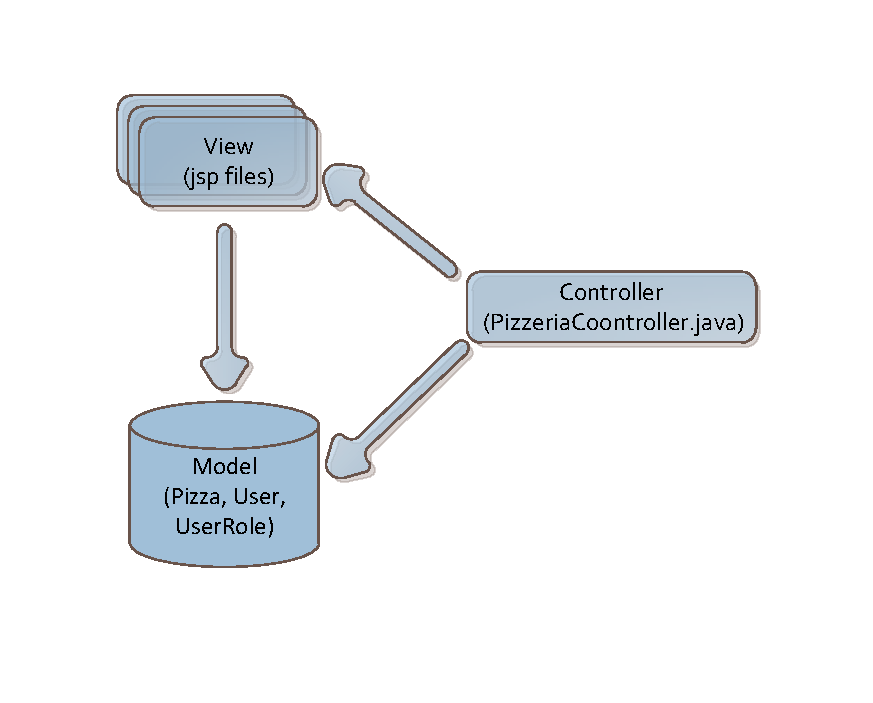
\includegraphics[width=0.6\textwidth]{fig/MVC_JSP.pdf}
        \caption{MVC for JSP}
        \label{fig.MVC_jsp}
    \end{center}
\end{figure}
The \emph{model} is represented by entities that access data from a MySql
database. In order to access data and persist application state we have based our model
design on the DAO (Data Access Object) pattern 
\href{http://java.sun.com/blueprints/corej2eepatterns/Patterns/DataAccessObject.html/}{here}\footnote{\url{http://java.sun.com/blueprints/corej2eepatterns/Patterns/DataAccessObject.html/}}.
It provides a technique for separating
object persistence and data access logic from any particular persistence
mechanism or API. We have used
\href{http://www.hibernate.org/}{Hibernate}\footnote{\url{http://www.hibernate.org/}}
- an object-relational mapping library, for mapping a
model to a relational database. Therefore, the persitance layer is implemented
using Hibernate and DAO pattern.\\\\
The \emph{dk.itu.ws.pizzeria.model} package contains the generic models (POJOs):
Pizza, User, UserRole. They are extended by hibernate specific implementation
in \emph{dk.itu.ws.pizzeria.model.hibernate}: HibernatePizza, HibernateUser,
HibernateUserRole. Besides the specific methods i=they also contain a method
for field validation and for displaying an error message. The DAO pattern is
illustrated in
\emph{dk.itu.ws,pizzeria.model.dao.*} packages. The \emph{HibernateGenericDAO}
contains the implementation of the main operations (add, update, remove, select)
on the database and it is extended for specific operations by
\emph{HibernateUserDAO} (findByEmail) and \emph{HibernateUserDAO}(findByName,
findAll).\\\\
The \emph{controller} \emph{PizzeriaController} in
\emph{dk.itu.ws.pizzeria.web} is a servlet that has the responsability to read
the request, invoke the data-access code to obtain results and store them (in
the request, session, servlet context) and forward the request to the JSP page
which is appropiate for the situation. A parameter stored in the request,
\emph{action}, is used to differenciate between the possible operations
that could happen.\\\\
The \emph{view} presents information and results in form of .jsp pages. We
have organized the views in 3 folders according to their relevance: admin -
which provides the views for adding/deleting a pizzas, auth - registration
and login, chart - view chart, add/remove pizzas, checkout.\\\\
In order to implement the mentioned requirements we have taken the following
decisions.\\\\
The field validations required for registering a
new user or adding a new pizza were implemented using a validate function and 
a get error messages function, in the \emph{HibernateUser} and \emph{HibernatePizza} classes.\\
\\\\
For authentication we have used the security built-in Tomcat using a
JDBCRealm. For a correct setup the server.xml has to be copied in
\url{CATALINA_HOME/conf} and the mysql\_connector jar in \url{CATALINA_HOME/lib}. In the web.xml file the
security constraints are specified /chart is secured to USER access only and /admin is secured to ADMIN access only.
The logged in user is kept in the session. We use form based
authentication which is automatically triggered every time a secure resource
is accessed and a user is not logged in. This approach is highly secure and the
application in easily portable to other containers supporting JAAS.
\\\\
We have used a HttpSessionAttributeListener - ChartAttributeListener and a
HttpSessionListener - LoginEventListener to handle the correct creation of the
shopping chart when specific events occur.
\subsubsection{JSF}
\label{sec.thesystem.jsf}
The implementation of the web shop using Java Server Faces was completed using
JSF 2.1.\\\\
The overall design follows the MVC pattern as illustrated in Figure
\ref{fig.MVC_jsf}. 

\begin{figure}[H]
    \begin{center}
        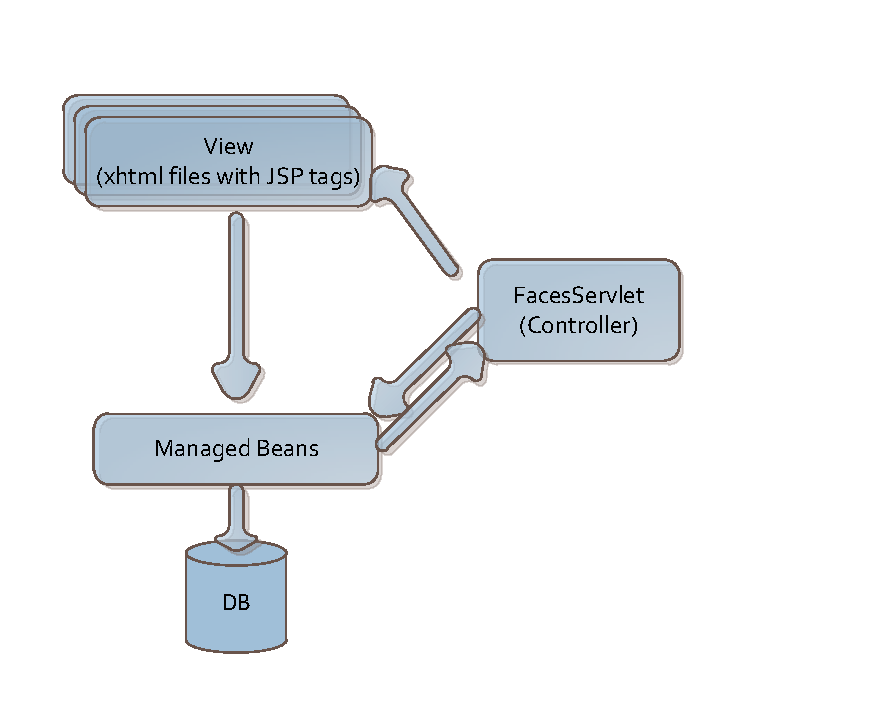
\includegraphics[width=0.6\textwidth]{fig/MVC_JSF.pdf}
        \caption{MVC for JSF}
        \label{fig.MVC_jsf}
    \end{center}
\end{figure}

The model consists of annotated beans. We have use Hibernate and DAO for the
persistance layer also in this case. For validation in this case we have used
Hibernate validator. We made use of
\href{http://blogs.sun.com/enterprisetechtips/entry/using_cdi_and_dependency_injection}{CDI}\footnote{\url{http://blogs.sun.com/enterprisetechtips/entry/using_cdi_and_dependency_injection}}
(Context Dependency Injection) support in JSF 2.1. It allows enterprise beans to act as managed beans in a JSF application. CDI services makes it a lot easier to build a Java EE web application 
that accesses a database with persistence. We have used a
\href{http://seamframework.org/Weld}{weld-servlet}\footnote{\url{http://seamframework.org/Weld}}
as an org.jboss.weld.environment.servlet.Listener to handle CDI (Context and
Dependency Injection) in Tomcat. This simplies the beasn.xml.
\\\\
The controller is FacesServlet and it is configured by faces-config.xml.
The navigation is implicit (the outcome of the action is the next view using the
extension of the current view) e.g. outcome success from register.xhtml will
lead to success.xhtml.
\\\\
For the view we have experimented with HTML5 and AJAX. We validate each field
just when the focus on that field is lost (with ajax calls). We used the
primefaces JSF library to augment the core feature and components. For the
common\_header a JSF template and UI composition was used.
\\\\
The authentication is simple: every time the user tries to enter a secured area
we prompt for the credentials. It was hard to implement resource based constraints 
(like with JSP) because almost all the control is in the controller. Anyhow, we
have looked in the Servlet3 specification where the underlying authentication 
mechanism can be programatically invoked from the servlet request, which would solve our problem
we have actually experimented with that also, but didn\'t finalize the approach.
\subsection{Usage of the system}
\label{sec.thesystem.usage}
In order to access the webshop the following links should be used:

\begin{itemize}
  \item JSP -
  \href{http://184.106.81.39:8080/LaPizzeria}{\url{http://184.106.81.39:8080/LaPizzeria};}
  \item JSF -
  \href{http://184.106.81.39:8080/LaPizzeriaJSF2/faces/index.xhtml}{\url{http://184.106.81.39:8080/LaPizzeriaJSF2/faces/index.xhtml};}
\end{itemize}

The server IP is 184.106.81.39 and the port 8080. In the Appendix
\ref{sec.appendix} a few screenshots illustrating the main functionalities can be found.
